\chapter{Concepts in Generative Models}

In machine learning, we can distinguish between two kinds of models:
\begin{enumerate}
    \item \textbf{Discriminative models} model $P(y|x)$. This means they focus on learning the \textbf{boundary} between classes. They learn how to determine or model $y$ given $x$. The most basic example of a discriminative model is one that classifies between positive and negative samples, and has to find a boundary as a function of the input data $x$.
    \item \textbf{Generative models} model $P(x,y)$, this is, they model the \textbf{distribution} of the data. If no labels or classes $y$ are available, they simply model $P(x)$. This means they create much richer representation of the underlaying data than discriminative models, which just focus on the boundaries (and can be very precise when modeling them). 
\end{enumerate}

This means that a generative model, when properly trained, needs to have a much deeper insight into what the data represents than a discriminative model, that will just focus on the part of the data that is needed to perform a specific task. Thus, a generative model will have potentially a higher amount of learned concepts to be able to represent all the data.

In the model we have been studying so far, the image network only needs to discriminate the image features that have some relation to the audio that describes them. If there are some visual concepts that are never described in the audio, the network will not need them to discriminate the positive audios from the negatives, so it will not model them. The same applies for the audio network: it will not need to model audio features that are not present in the image. While this may seem a limitation for the system, it is not really an issue: if an image feature is consistently ignored in the audio, it means it does not represent a concept humans consider important.

In this chapter, we will study how generative models, and more specifically \ac{GAN}, represent concepts, and how can we detect those concepts and relate them to speech.

\section{How modify the generated content of GANs\footnote{The explanation in this section is not my work. It is originally done using natural images, and it is work in progress. I just applied it to the CLEVR dataset, which can give us future insights into how to improve the current results, as well as giving us numeric and objective metrics.}}

In order to understand the chapter, a brief explanation is needed on how to modify the content of GANs.

\section{Discovering concepts using captions}

Two different networks means two different systems that have learned different things. GAN te conceptes visuals, i la altra els vol descobrir a traves de l'audio.

Idees futures: loop en que la gan no estigui frozen i tambe s'adapti a entendre els detalls que l'audio dona (a mesura que apren, els usuaris de mechanical turk van refinant i tal i qual).
\begin{figure}
    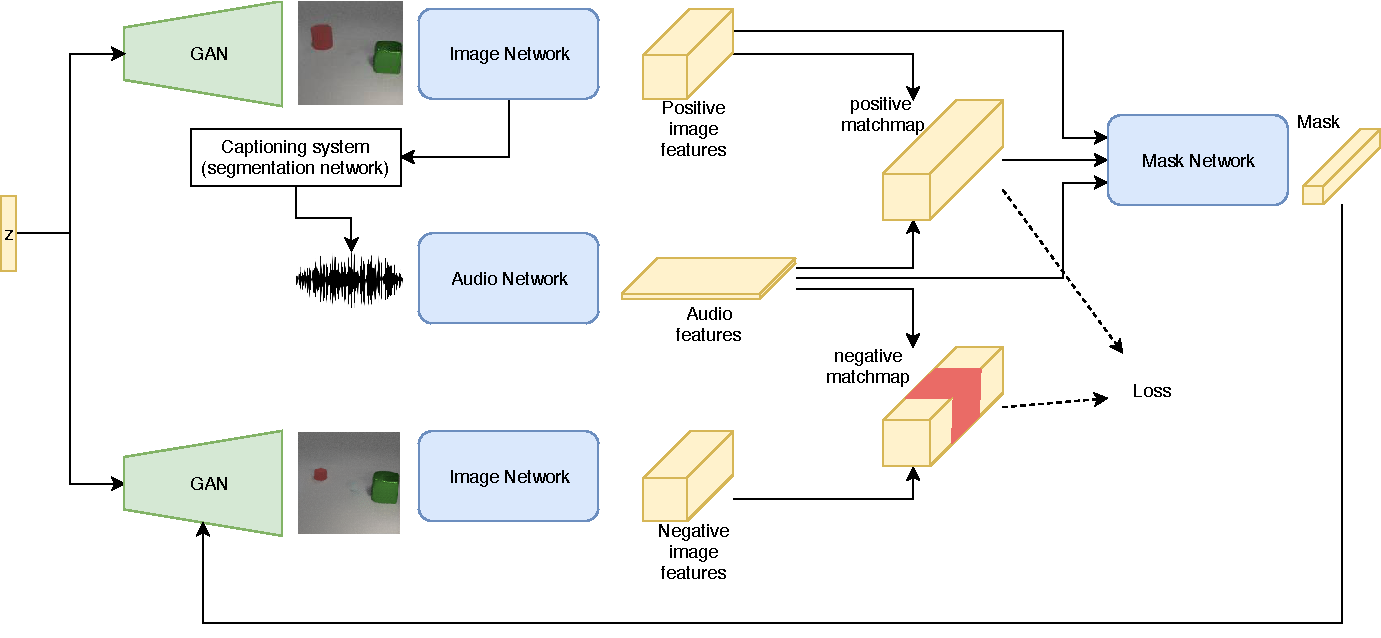
\includegraphics[width=1\linewidth]{figures/GANsandaudio.pdf}
%\vspace{-.3in}
    \caption[Caption]{Caption}
    \label{fig:ganaudio}
\end{figure}
